\subsection{Two Transistor Circuits}
Before you go onto this section, make sure you fully grasp the idea behind the single transistor circuits. 
\subsubsection{Current Mirror}
\begin{figure}[H]
    \centering
    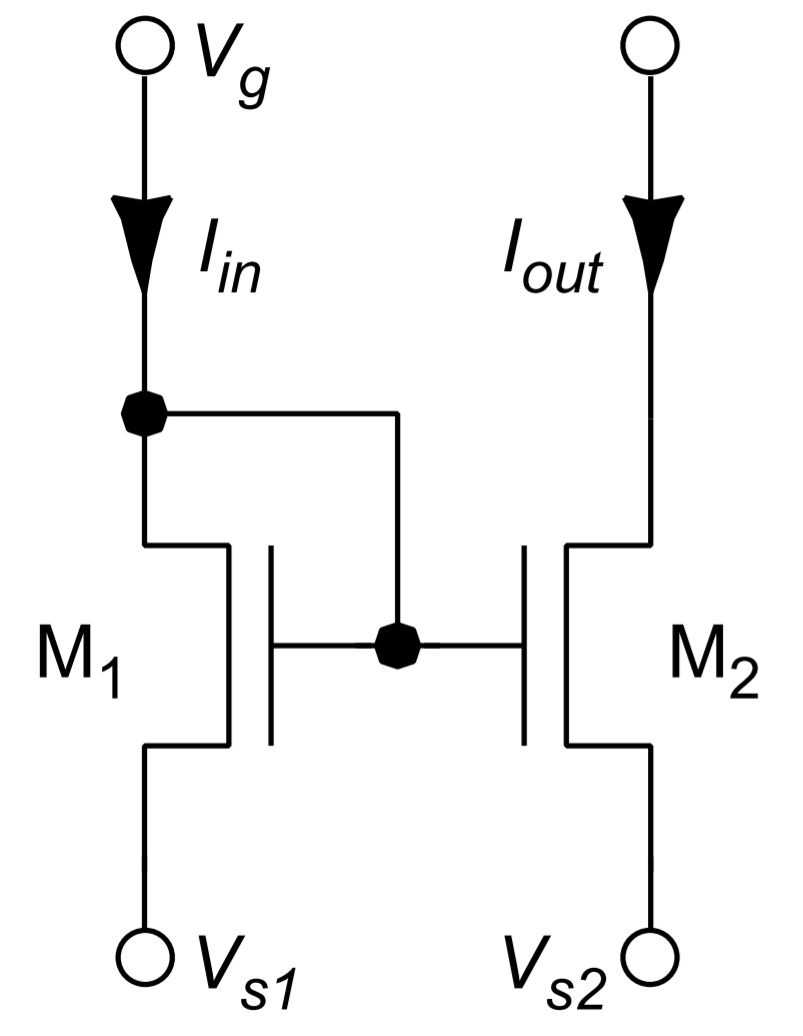
\includegraphics[width=0.3\linewidth]{../../Figures/Current_Mirror.PNG}
    \caption{Current Mirror. Adapted from Lecture Notes.}
    \label{fig:N-Type Current Mirror}
\end{figure}
In this circuit, the output current is a \emph{mirrored copy} of the input current. What does this mean? Suppose both nFETs M1 and M2 1) have the same source voltage, 2) have the same size (so weird difference due to device mismatch don't apply) and 3) are in saturation. Remember from the previous section that the current $I_{in}$ flowing through the Diode-Connected transistor M1 sets the gate voltage. You can also see that both M1 and M2 share the same gate voltage. Thus, given the assumptions taken, we reach a circuit where $I_{in}$ sets $I_{out}$ of M2. What's most interesting is that we can also scale the output current $I_{out}$ by setting difference source voltages $V_{s1}$ and $V_{s2}$, or by having different transistor sizes. Let's derive the equation when we have different source voltages: 
\begin{equation}
For M1: I_{in} = I_{n0} e^{\frac{\kappa_{n}V_g - V_{s_1}}{U_T}} = I_{n0} e^{\frac{\kappa_{n}V_g }{U_T}}e^{\frac{-V_{s_1}}{U_T}}
\end{equation}
\begin{equation}
For M2: I_{out} = I_{n0} e^{\frac{\kappa_{n}V_g - V_{s_2}}{U_T}} = I_{n0} e^{\frac{\kappa_{n}V_g }{U_T}}e^{\frac{-V_{s_2}}{U_T}}
\end{equation}
\begin{equation}
I_{n0} e^{\frac{\kappa_{n}V_g }{U_T}} = \frac{I{in}}{e^{\frac{-V_{s_1}}{U_T}}} = \frac{I{out}}{e^{\frac{-V_{s_2}}{U_T}}}
\end{equation}
\begin{equation}
Thus, I_{out} = I_{in} e^{\frac{V_{s_1} - V_{s_2}}{U_T}}, \ with \ Gain \ M = e^{\frac{V_{s_1} - V_{s_2}}{U_T}}
\end{equation}

We can also write the equation for same source voltage but different transistor size, without going into the derivation we reach: 

\begin{equation}
I_{out} = M I_{in} \ with \ Gain \ M = \frac{W_2/L_2}{W_1/L_1}
\end{equation}

\newline \newline
\textbf{P-Type Current Mirror} \\

A common exam question is to draw the P-type equivalent circuits of circuits we've learned. It also turns out that the P-type current mirror will be particularly important when studying the transconductance amplifier, so let's take some time to briefly study its behaviour.   

\begin{figure}[H]
    \centering
    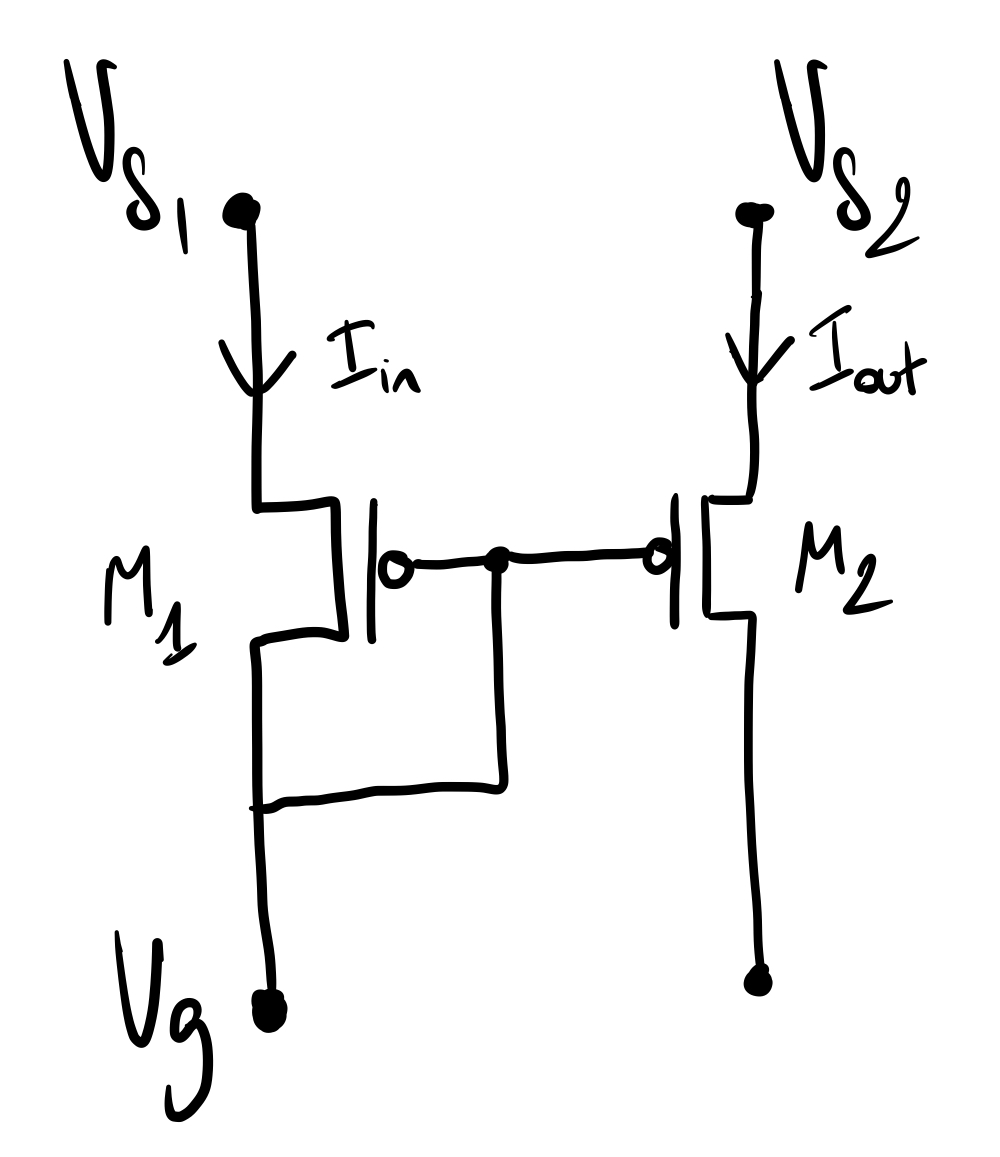
\includegraphics[width=0.3\linewidth]{../../Figures/Ptype_Current_Mirror.jpg}
    \caption{P-Type Current Mirror. Adapted from my brain lol.}
    \label{fig:N-Type Current Mirror}   
\end{figure}

The P-type current mirror works just like the N-type, but in reverse. In the N-type current mirror, we \textit{diode connect} the drain of the first transistor, \textit{at higher potential}, to the gate, thereby ensuring saturation. In an PFET, this is the opposite, we \textit{diode connect} the drain of the first transistor, \textit{at lower potential}, to the gate. This tiny difference ends up yielding the exact same output equation for $I_{out}$. 

\subsubsection{Intrinsic Voltage Gain}

In the previously derived current mirror, a gain has been evidenced between the input current and the output current: that means that we manage to scale the \textit{current} by a certain constant value that we have control over when designing our circuit. This is very useful in a lot of different applications and circuits that will be derived next. It also is very useful to be able to scale \textit{voltage}!

\begin{figure}[H]
    \centering
    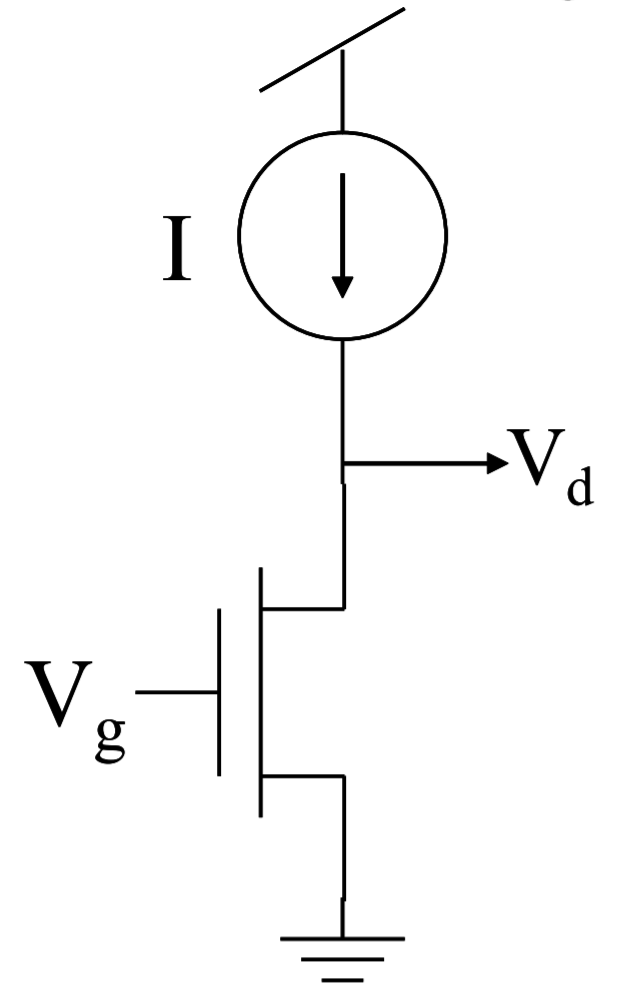
\includegraphics[width=0.3\linewidth]{../../Figures/Intrinsic_Voltage_Gain_Transistor.PNG}
    \caption{Intrinsic Voltage Gain with Transistors. Adapted from Lecture Notes.}
    \label{fig:basalandcerebellum}
\end{figure}

The first thing to note in this figure is the current source. We've seen them before, but this one is slightly different: it's a pFET current source (remember I made a comment about pFET current source being most often used!). The source voltage $V_s$ is at $V_{dd}$ and the drain voltage is $V_d$. Current flows from positive to negative, so from top to bottom (current, not electrons - thanks again Benjamin Franklin). Note again that this allows to have a \emph{constant} current flowing. We can evalute the gain of this circuit as follows: 

\begin{equation}
    \mathrm{Gain \ A} = \frac{\partial V_d}{\partial V_g} = \frac{\partial I}{\partial V_g}\frac{\partial V_d}{\partial I} = \frac{g_m}{g_d} \footnote{We have defined transistor conductance in chapter 3.} = \frac{\kappa V_E}{U_T}
\end{equation}

The voltage gain is thus set by tweaking $\kappa$, Early voltage $V_E$ and thermal voltage $U_T$.

\subsubsection{Source Follower}

\begin{figure}[H]
    \centering
    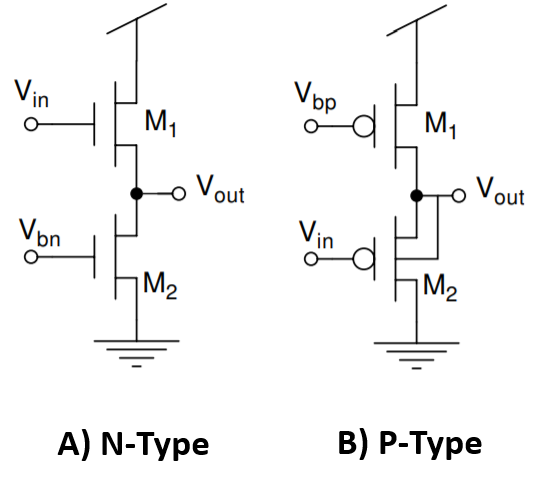
\includegraphics[width=0.5\linewidth]{../../Figures/Source_Follower.PNG}
    \caption{Source Follower circuits. A) N-Type Source Follower. B) P-Type source Follower. Adapted from Lecture Notes.}
    \label{fig:basalandcerebellum}
\end{figure}

The source-follower circuit linearly transforms a voltage at a high-impedance input terminal into a voltage at a lower-impedance output terminal, such that the output signal is able to drive larger loads than the input signal. It is constructed by connecting a fixed current source to the source of a MOSFET operated in saturation. 
\newline \newline
\textbf{N-Type Source Follower:} 
\\
In figure 13.A, we can see a N-Type source follower. $M_{2}$ is the NFET current source and $M_{1}$ is the input transistor. The input voltage $V_{in}$ is applied to the gate voltage of $M_1$ and the output voltage $V_{out}$ is the source voltage of $M_1$. In the subtreshold domain, assuming both transistors are in saturation regime, we can derive the following equations describing the behaviour of the circuit:  

\begin{equation}
I_{M1} = I_{n0}e^{\kappa_n V_{in}/U_T - V_{out}/U_T}
\end{equation}
\begin{equation}
I_{M2} = I_{n0}e^{\kappa_n V_{bn}/U_T - V_{s_{M_2}}/U_T} = I_{n0}e^{\kappa_n V_{bn}/U_T} \ as \ V_{s_{M_2}} = 0
\end{equation}
Because the two transistors are connected in series, $I_{M1} = I_{M2}$, we can therefore reach by rearranging:
\begin{equation}
V_{out} = \kappa_n(V_{in} - V_{bn}) \ with \ V_{out} > 4U_T \ to \ keep \ M_2 \ in \ saturation.
\end{equation}
What we get is thus an output voltage which follows the input voltage, and can be scaled with the gate voltage from the current source that we connect it with.
\newline \newline
\textbf{P-Type Source Follower:} \
\\
In figure 13.B, we can see a P-Type source follower. The logic and objective of the circuit are pretty much the same as the NFET version, but with a PFETs.  $M_{1}$ is the PFET current source and $M_{2}$ is the input transistor. An important difference here is that $V_{out}$ is connected to the bulk of $M_2$. Remember from the chapter 2 section on bulks, wells and biasing that MOSFETs are typically biased to $V_{dd}$ or $V_{ss}$ at their bulk. Here, they are biased to $V_out$.  Let's go through it: HERE THERE IS SOMETHING BOTHERING ME WITH THE EQUATION OF THE PFET, WHICH IS SLIGHTLY DIFFERENT WITH THE BULK CONNECTED TO $V_OUT$ BUT WHERE IS THIS EXPLAINED? APPARENTLY WHEN YOU DON'T HAVE THAT CONFIGURATION, YOU KEEP THE KAPPA IN THE EQUATION? HOW? 

ALSO THIS BIt, PAGE 131 OF THE TEXTBOOK EXPLAINS THE IDEA: 
It is possible to get around the $\kappa$ reduction factor in the transfer characteristic, if the bulk potential of the input MOSFET can be controlled independently. As mentioned previously, in a CMOS process this independence is possible for only one type of MOSFET: The one that sits in a well with opposite doping from the substrate.

\begin{equation}
I_{M1} = I_{p0}e^{-\kappa_p(V_{bp} - V_{dd})/U_T}
\end{equation}
\begin{equation}
I_{M2} = I_{n0}e^{-\kappa_p(V_{in} - V_{out})/U_T}
\end{equation}
Because the two transistors are connected in series, $I_{M1} = I_{M2}$, we can therefore reach by rearranging:
\begin{equation}
V_{out} = (V_{dd} - V_{bp}) + V_{in} \ with \ V_{out} < V_{dd} - 4U_T \ to \ keep \ M_1 \ in \ saturation.
\end{equation}

Notice how we got rid of the $\kappa$ here, where $V_{out}$ is now linear with the input. This variation of the source follower is called a \textit{unity gain} source follower. What's the point of this circuit though? Why would you want to have an output equal to the input? Why should you go through the trouble of building identity. The reason, according to Giacomo, is to \textbf{decouple} the left side from the right side. You might have noise, load or capacitance on one side and you don't want to influence the rest of the circuit with that and keep it clean. You could also use it, as in the previous nFET source follower, use it to shift by some value the $V_{out}$ compared to $V_{in}$.
